\chapter{Evaluation}
\label{ch:evaluation}
To evaluate the proposed solution, firstly, it was tested against standard test cases, secondly, it was compared against XTurtle framework, lastly, it was validate with arbitrary large RDF files. This chapter discusses all of such details in the following text. 

\section{Experiment 1: Validating with RDF Suite Test}

The evaluation phase finds its starting point at \citealp{TurtleTests:Online} where Test Suite files of Turtle serialization are found. Any new parser (focused on the same RDF serialization) can its proficiency be validated against these files. Files at \cite{TurtleTests:Online} are recommended by W3 Consortium\footnote{\href{https://www.w3.org/}{W3 Consortium}} to validate a parser that parses a Turtle format.  




\begin{table}[]
\centering
\begin{tabular}{|l|l|l|l|}
\hline
\begin{tabular}[c]{@{}l@{}}Error Type Classification \end{tabular} & Detected & \begin{tabular}[c]{@{}l@{}}Not detected\end{tabular} & Total \\ \hline
 Escape Characters              &      0    &    4 &   4  \\ \hline
 Bad Keywords             &      5   &    0 &   5  \\ \hline
 Bad Literals with langTag             &      2   &    0 &   2  \\ \hline
 Bad Local Name-space in IRI             &      2   &    3  &   5  \\ \hline
 Bad Namespace in IRI             &      2   &    0 &   2  \\ \hline
 N3 Extra             &      11   &    1 &   12  \\ \hline
 Bad Namespace in Directives             &      2   &    0 &   2  \\ \hline
 Bad Number as a Literal             &      5   &    0 &   5  \\ \hline
 Bad Directives             &      4   &    0 &   4  \\ \hline
 Bad Strings             &      6   &    1 &   7  \\ \hline
 Bad Structures            &      12   &    0 &   12  \\ \hline
 Bad IRI            &      2   &    3 &   5  \\ \hline
 Total            &      53   &    12 &   65  \\ \hline
\end{tabular}
\caption{\textbf{Evaluation of RDF-Doctor against Detection of Incorrect Syntax in Turtle Test Suite \cite{TurtleTests:Online}.} The test focused on the files, included with an incorrect Turtle syntax}
\end{table}
\begin{table}[]
\centering
\begin{tabular}{|l|l|l|l|l|}
\hline
\begin{tabular}[c]{@{}l@{}}File Content \end{tabular} & Detected & \begin{tabular}[c]{@{}l@{}}Not detected \\ without errors \end{tabular} &\begin{tabular}[c]{@{}l@{}} Not detected \\ with errors \end{tabular}  & Total \\ \hline
 Correct Syntax              &      185    &    0 &   25  & 210 \\ \hline
 Incorrect/Bad Syntax              &      53    &    12 &   0  & 65 \\ \hline
 Total            &      238   &    12 &   25 & 275  \\ \hline
\end{tabular}
\caption{\textbf{Summary Evaluation of RDF-Doctor for both Correct and Incorrect Syntax in Turtle Test Suite \cite{TurtleTests:Online}.} }
\end{table}


The test summarized the result when dealing with correct and incorrect Turtle syntax, for a correct syntax, it should be recognized as correct, but in the table when can see that there are some correct syntaxes but  RDF-Doctor shows some errors, for an incorrect syntax, it should be detected as an incorrect syntax and an error should be fired, again, in the table values of column "No detected without errors", those are value for incorrect syntexes but RDF-Doctor does not consider them as wrong and as well no errors were fired

For evaluation, the precision and recall are computed using the equations \ref{eq:1} and \ref{eq:2} respectively.  
\begin{align} 
   Precision=  \frac{t_p}{t_p+f_p} \label{eq:1}
\end{align}
\begin{align}
   Recall =  \frac{t_p}{t_p+f_n} \label{eq:2}
\end{align}

\begin{figure}[ht]
\begin{center}
		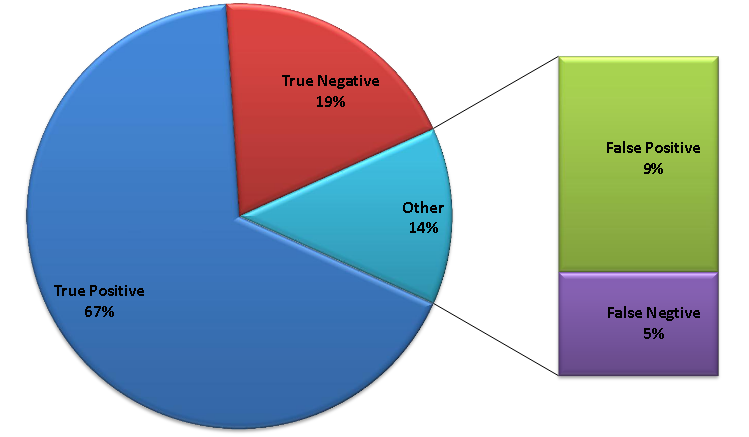
\includegraphics[scale=0.5,angle=0]{images/PieChartExperiment1.png}

		\label{Fig:pieChartExperiment1}
		\caption{\textbf{Pie Chart summarizes RDF-Doctor Evaluation based using Turtle Test Suite \cite{TurtleTests:Online} }}
\end{center}
\end{figure}

\section{Experiment 2: Random Syntax Errors Generation}

In this experiment, number of syntax errors are arbitrarily created using a Poisson Distribution, for example. a user who is working on on RDF data for 8 hours and each one hour he is making a change (insert/modify/delete a text) is simulated. The average number of making syntax errors per time interval is represented by the parameter $\lambda$ . To make more clear, if   $\lambda$ = 5, it means that five syntax errors were occurred per hour.  Assuming a user can introduce 10 syntax error per hour

	\begin{figure}[ht]
	\begin{center}
		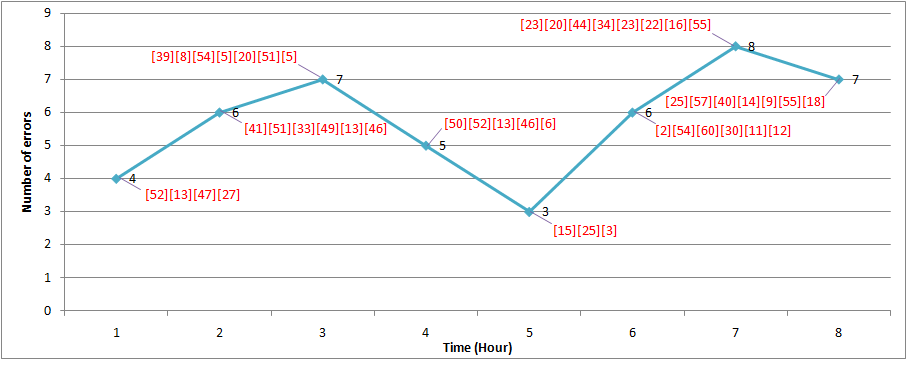
\includegraphics[scale=0.58,angle=0]{images/experiment2.png}
				\setlength\belowcaptionskip{-5mm}
		\caption{\textbf{Random Syntax Errors Distribution.} Number and types of syntax errors between brackets for a user in an interval of 8 hours. A Possion distribution with $\lambda$ = 5 models an average of 5 syntax errors per hour. A uniform distribution is computed to represent the type of errors} 
		\label{Fig:experiment2}
	\end{center}
\end{figure}

\section{Experiment 3: Impact of Numbers of Errors and RDF Volume on Performance}

To evaluate the performance of the proposed solution, this experiment will be held where number of syntax errors and RDF input data are varied. Two types of anthologies are used: small and medium size ones.  
%\section{Accuracy}

%\section{Scalability}








